\subsection{Experimental Results on Multivariate Imputation Methods}
%\subsubsection{Multivariate TR-MF}
%weilun please double check this section

%more?

\begin{figure*}[h]
\centering
%\subfigure[]
%{
%	\label{fig:multi_berkeley_random_hum}
%	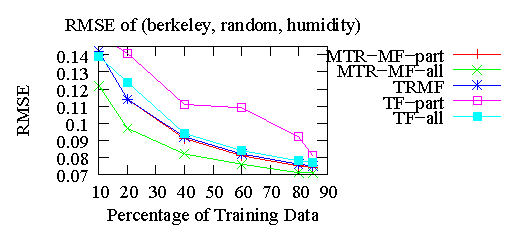
\includegraphics[scale=1]{berkeley_random_humidity_pspdftex.eps}
%}
%\hspace{0in}
%\subfigure[]
%{
%	\label{fig:multi_berkeley_random_tem}
%	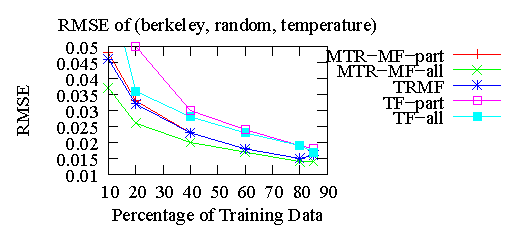
\includegraphics[scale=1]{berkeley_random_temperature_pspdftex.eps}
%}
%\hspace{0in}
%\subfigure[]
%{
%	\label{fig:multi_berkeley_temporal_hum}
%	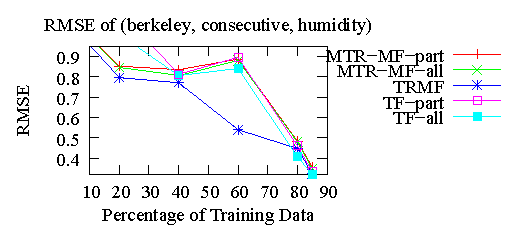
\includegraphics[scale=1]{berkeley_temporal_humidity_pspdftex.eps}
%}
%\hspace{0in}
%\subfigure[]
%{
%	\label{fig:multi_berkeley_temporal_tem}
%	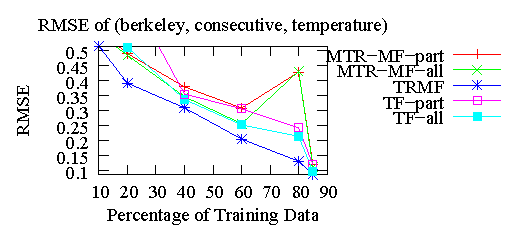
\includegraphics[scale=1]{berkeley_temporal_temperature_pspdftex.eps}
%}
\subfigure%[]
{
	\label{fig:multi_traffic_random_hum}
	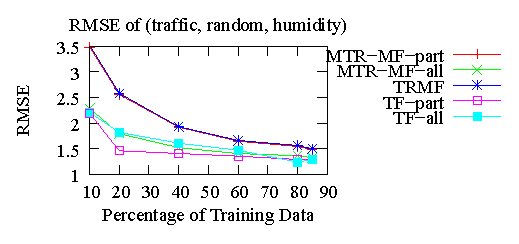
\includegraphics[width=4.3cm, height=2.2cm, trim=20 0 0 0, clip]{traffic_random_humidity_pspdftex.eps}
}
\hspace{-0.4cm}
\subfigure%[]
{
	\label{fig:multi_traffic_random_tem}
	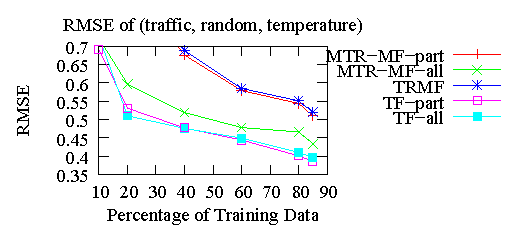
\includegraphics[width=4.3cm, height=2.2cm, trim=20 0 0 0, clip]{traffic_random_temperature_pspdftex.eps}
}
\hspace{-0.4cm}
\subfigure%[]
{
	\label{fig:multi_traffic_temporal_hum}
	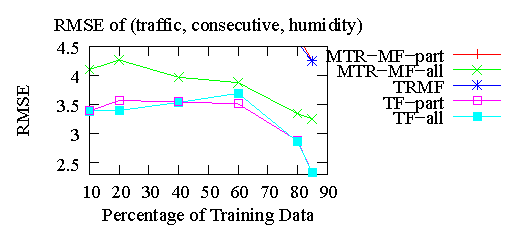
\includegraphics[width=4.3cm, height=2.2cm, trim=18 0 0 0, clip]{traffic_temporal_humidity_pspdftex.eps}
}
\hspace{-0.4cm}
\subfigure%[]
{
	\label{fig:multi_traffic_temporal_tem}
	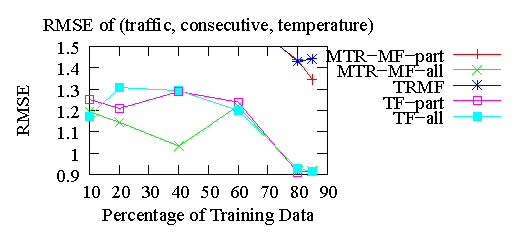
\includegraphics[width=4.3cm, height=2.2cm, trim=13 0 0 0, clip]{traffic_temporal_temperature_pspdftex.eps}
}
\vspace{-0.1in}

\caption{\label{fig:multi}
Root mean square errors of multivariate models, varying the percentage of training data.
The units of measurement are Celsius for temperature and \% for humidity.
}

\vspace{-0.4cm}
%\hspace{0in}
%\caption{}
\end{figure*}
















%\begin{table*}
%%
%\begin{tabular}{cc}
%\subfigure[A]{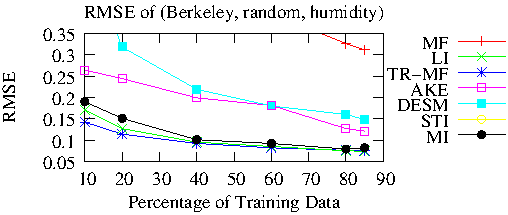
\includegraphics[scale=1]{table2_BRH}} 
%   & \subfigure[B]{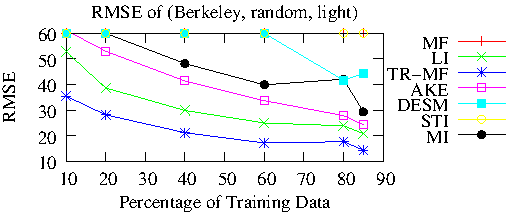
\includegraphics[scale=1]{table3_BRL}}\\
%\end{tabularx}
%\end{table*}
%\end{figure}
%\begin{figure}[H]
%\centering
%\mbox{
%\input{table11.pspdftex}}
%\caption{RMSE of (traffic, temporal, temperature}
%\end{figure}


To evaluate multivariate imputation models, in the experiments we allow temperature and humidity information to mutually enhance the predictions.
Here we compare the two proposed multivariate imputation models: MTR-MF and TR-TF with the univariate model TR-MF, which has been demonstrated to outperform other models in the previous section. 

There are two different scenarios we are concerned with in this experiment.
For illustration purposes, assume the goal is to predict the missing entries in the temperature matrix.
In the first scenario (denoted as MTR-MF-all and TR-TF-all), we do not cover up the humidity data and use this data in its entirety.
The goal here is to evaluate whether using all the humidity information allows our model to improve the temperature predictions.
In the second scenario (denoted as MTR-MF-part and TR-TF-part), we assume the humidity readings are missing together whenever temperature readings are missing.
Note that such cases happen quite often in WSN due to communication loss or sensor node malfunction.
In the second scenario, MTR-MF-part can be performed without problems.
However, to predict an entry in the temperature matrix, the TR-TF model requires use of the corresponding entry in the humidity matrix.
In the TR-TF-part, such issues can be addressed by first predicting the missing humidity readings based on the humidity TR-MF model, and then apply TR-TF.

The results are shown in Figure~\ref{fig:multi}.
Except MTR-MF-part, which remains similar performance as TR-MF, we see significant improvement on TR-TF-all, TR-TF-part and MTR-MF-all. 
From this we see the effect of heterogeneous information and we can conclude that:
although MTR-MF is not helpful when multiple sensors are missing together,
both of the temperature and humidity information can indeed be used to enhance the prediction of the other.
%
%With focus on the TR-TF model, we first observe that TR-TF-part and TR-TF-all produce results of similar quality.
%The results further show that the TR-TF model outperforms all other models significantly for the traffic dataset, but performs less well for the Berkeley dataset.
%We believe the reason for this different is as the follows.
%To perform TR-TF, it is required that each dimension of the tensor be discretized.
%While the sensor and time-step dimensions are already discretized, the third dimension (i.e., humidity or temperature) is not.
%Therefore we need to perform discretization before conducting tensor factorization.
%The problem for the Berkeley dataset is that as an indoor dataset, the variances in temperature and humidity readings are not as large as those of the traffic dataset, therefore a uniform discretization would lead to an uneven split of values across this third dimension, which then limits its power in explaining the data.
% 
%As for the MTR-MF model, the results show that MTR-MF-part does not outperform TR-MF, but MTR-MF-all does (except for the consecutively missing Berkeley dataset).
%We may conclude that the MTR-MF model is not helpful when multiple sensors are missing together, but is likely to be useful when the heterogeneous signal is fully available.

%\redtext{don't use result here!!! see my google doc!}
%\begin{table}[htbp]
%\setlength{\tabcolsep}{2pt}
%\centering
%\caption{Multivariate RMSE (Berkeley, random)}
%\label{table:multi_berkeley_random}
%\begin{tabular}{r | r r r r r}
%train	&TR-MF	&MtMF-Train	&MtMF-all &TF-Train & TF-all \\ \hline
%humid10\%	&0.1424	&0.1420	&0.1222 &0.510&0.1392\\
%humid20\%	&0.1135	&0.1135	&0.0973&0.1412&0.1243\\
%humid40\%	&0.0916	&0.0909	&0.0822&0.1113&0.0944\\
%humid60\%	&0.0817	&0.0806	&0.0758&0.1086&0.0842\\
%humid80\%	&0.0757	&0.0748	&0.0709&0.0918&0.0781\\
%humid85\%	&0.0751	&0.0739	&0.0712&0.0812&0.0772\\ \hline
% temp10\%	&0.1137	&0.1148	&0.0729&0.0878&0.0701\\
% temp20\%	&0.0462	&0.0481	&0.0369&0.0501&0.0361\\
% temp40\%	&0.0316	&0.0328	&0.0263&0.0303&0.0280\\
% temp60\%	&0.023	&0.0232	&0.0201&0.0243&0.0234\\
% temp80\%	&0.0182	&0.0183	&0.0166&0.0193&0.0186\\
% temp85\%	&0.0153	&0.0154	&0.0143&0.0175&0.0171\\
%\end{tabular}
%\end{table}
%
%\begin{table}[htbp]
%\setlength{\tabcolsep}{2pt}
%\centering
%\caption{Multivariate RMSE (Berkeley, temporal)}
%\label{table:multi_berkeley_temporal}
%\begin{tabular}{r | r r r r r}
%train	&TR-MF	&MtMF-Train	&MtMF-all &TF-Train&TF-all \\ \hline
%humid10t	&0.957&0.996& 	0.991&1.110&1.291\\
%humid20t	&0.796&0.852& 	0.846&1.127&1.009\\
%humid40t	&0.771&0.835& 	0.807&0.813&0.806\\
%humid60t	&0.540&0.887& 	0.880&0.896&0.841\\
%humid80t	&0.447&0.483& 	0.480&0.461&0.406\\
%humid85t	&0.323&0.356& 	0.348&0.332&0.321\\	\hline
% temp10t	&0.515&0.567& 	0.555&1.525&1.109\\
% temp20t	&0.392&0.491& 	0.485&0.705&0.512\\
% temp40t	&0.310&0.380& 	0.347&0.356&0.338\\
% temp60t	&0.206&0.309& 	0.257&0.307&0.253\\
% temp80t	&0.132&0.429& 	0.432&0.243&0.215\\
% temp85t	&0.088&0.122& 	0.114&0.121&0.099\\
%\end{tabular}
%\end{table}
%
%\begin{table}[htbp]
%\setlength{\tabcolsep}{2pt}
%\centering
%\caption{Multivariate RMSE (traffic Data, Random)}
%\label{table_multi_traffic_random}
%\begin{tabular}{r | r r r r r}
%train	&TR-MF	&MtMF-Train	&MtMF-all &TF-train & TF-all\\ \hline
%humid10\%	&3.524 	&3.486 	&2.291&2.190&2.209\\  
%humid20\%	&2.583 	&2.558 	&1.796&1.461&1.821\\
%humid40\%	&1.932 	&1.921 	&1.523&1.409&1.609\\
%humid60\%	&1.664 	&1.649 	&1.408&1.357&1.472\\
%humid80\%	&1.565 	&1.546 	&1.366&1.292&1.241\\
%humid85\%	&1.503 	&1.489 	&1.326&1.291&1.289\\ \hline
% temp10\%	&1.214 	&1.201 	&0.722&0.641&0.727\\
% temp20\%	&0.898 	&0.881 	&0.597&0.531&0.510\\
% temp40\%	&0.689 	&0.676 	&0.519&0.429&0.419\\
% temp60\%	&0.585 	&0.579 	&0.478&0.389&0.411\\
% temp80\%	&0.551 	&0.544 	&0.466&0.401&0.410\\
% temp85\%	&0.520 	&0.510 	&0.434&0.372&0.396\\
%\end{tabular}
%\end{table}
%
%\begin{table}[htbp]
%\setlength{\tabcolsep}{2pt}
%\centering
%\caption{Multivariate RMSE (traffic Data, temporal)}
%\label{table_multi_traffic_temporal}
%\begin{tabular}{r | r r r r r}
%train	&TR-MF	&MtMF-Train	&MtMF-all &TF-Train &TF-all\\ \hline
%humid10\%	&5.195 	&5.346 	&4.103&3.391&3.389\\  
%humid20\%	&5.487 	&5.565 	&4.263&3.571&3.399\\
%humid40\%	&5.782 	&6.009 	&3.968&3.544&3.537\\
%humid60\%	&4.954 	&4.918 	&3.877&3.512&3.694\\
%humid80\%	&4.564 	&4.700 	&3.346&2.881&2.862\\
%humid85\%	&4.248 	&4.248 	&3.254&2.329&2.332\\ \hline
% temp10\%	&1.700 	&1.708 	&1.194&1.251&1.173\\
% temp20\%	&1.812 	&1.815 	&1.144&1.209&1.307\\
% temp40\%	&1.832 	&1.835 	&1.033&1.288&1.293\\
% temp60\%	&1.666 	&1.646 	&1.220&1.239&1.201\\
% temp80\%	&1.430 	&1.437 	&0.916&0.911&0.929\\
% temp85\%	&1.441 	&1.345 	&0.915&0.912&0.912\\
%\end{tabular}
%\end{table}
%\subsubsection{Tensor Factorization} % need to be combined with multi TR-MF 

%We compare our TF method with models not incorporating heterogeneous sensor correlations in this section.
%Table ? and ? show the TF result of random split and temporal split on Berkeley dataset while table ? and ? show the TF result of random split and temporal split on traffic dataset.

\subsection{Designing Prediction Models after Imputation}\label{subsec:furtherPredict}
As stated previously, one main reason to conduct data imputation is that most off-the-shelf data analysis tools cannot deal with inputs with missing values.
Here one practical question to ask is: ``Can an improved imputation outcome indeed lead to the development of a better analysis model?''
Here we conduct an experiment using the {\em humidity} values of 20 sensors in the traffic dataset to build two regression models (linear regression and support-vector regression) in order
to predict the {\em temperature} values of the gateway.

In the experiment, we first remove the gateway signal from the matrix, and use TR-MF as well as the other competitive models (including LI and AKE) to fill in all the missing humidity values in the remaining 20 sensors.
Then for each imputation model, we use the filled-in readings of these 20 sensors as the inputs X and the gateway temperature values as the output Y to train the regression models for prediction.
We divide the data randomly into 80\% training and 20\% testing, and show the results of both regression models in Table \ref{table:gateway prediction}.
We use Mean Square Error~(MSE) to measure the error here and show the 95\% confidence interval.
The results confirm our hypothesis that a better imputation model does lead to the production of a better prediction models, and TR-MF again outperforms the other models in this respect.

%\begin{table} [htbp]
%\caption{Building Temperature Models Using Filled Humidity Data } \label{table:gateway prediction}
%\setlength{\tabcolsep}{2pt}
%\centering
%\small
%\begin{tabular} {c | r r r r | r r r r}
%& \multicolumn{4}{ c|}{LR} & \multicolumn{4}{|c}{SVR}  \\ \hline
%train & \begin{turn}{65}Mean\end{turn} & \begin{turn}{65}LI\end{turn} & \begin{turn}{65}AKE\end{turn}& \begin{turn}{65}TR-MF\end{turn}& \begin{turn}{65}Mean\end{turn} & \begin{turn}{65}LI\end{turn} & \begin{turn}{65}AKE\end{turn}& \begin{turn}{65}TR-MF\end{turn}  \\ \hline
%   10\%   &6.021&4.973&3.812&3.001   &6.222&5.012&4.101&3.144\\
%   20\%   &5.086&4.385&3.722&2.943    &5.524&4.551&3.972&2.807\\
%   40\%    &4.992&4.180&3.158&2.964     &5.281&4.241&3.244&2.877\\
%   60\%    &4.978&4.075&2.822&2.570     &5.003&4.175&3.058&2.692\\
%   80\%    &4.642&3.868& 2.874&2.526 &4.502&3.713& 2.891&2.681\\ 
%   85\%   &4.497&3.799&2.796&2.512      &4.323&4.018&2.895&2.409\\
%\end{tabular}
%\end{table}



\begin{table} [htbp]
\vspace{-0.2cm}
\caption{Accuracy of Temperature Models Built Using Filled Humidity Data } \label{table:gateway prediction}
\vspace{-0.2cm}
\setlength{\tabcolsep}{2pt}
\centering
\scriptsize
\begin{tabular} {c | c c c | c c c}
MSE& \multicolumn{3}{ c|}{Linear Regression} & \multicolumn{3}{|c}{Support Vector Regression}  \\ \hline
train & LI & AKE& TR-MF& LI & AKE& TR-MF  \\ \hline

10\%	&24.7 	\tiny$\pm{5.3}$	&14.5 	\tiny$\pm{7.8}$	&$\mathbf{9.0}$ 	\tiny$\pm{5.7}$	&25.1 	\tiny$\pm{5.9}$	&16.8 	\tiny$\pm{7.4}$	&$\mathbf{9.9}$ 	\tiny$\pm{5.9}$\\ 
20\%	&19.2 	\tiny$\pm{1.1}$	&13.9 	\tiny$\pm{3.1}$	&$\mathbf{8.7}$ 	\tiny$\pm{1.9}$	&20.7 	\tiny$\pm{1.5}$	&15.8 	\tiny$\pm{2.4}$	&$\mathbf{7.9}$ 	\tiny$\pm{2.2}$\\
40\%	&17.5 	\tiny$\pm{1.9}$	&10.0 	\tiny$\pm{2.2}$	&$\mathbf{8.8}$ 	\tiny$\pm{1.7}$	&18.0 	\tiny$\pm{1.6}$	&10.5 	\tiny$\pm{2.2}$	&$\mathbf{8.3}$ 	\tiny$\pm{1.9}$\\
60\%	&16.6 	\tiny$\pm{0.6}$	&8.0 	\tiny$\pm{1.3}$	&$\mathbf{6.6}$ 	\tiny$\pm{0.8}$	&17.4 	\tiny$\pm{0.7}$	&9.4 	\tiny$\pm{1.0}$	&$\mathbf{7.2}$ 	\tiny$\pm{0.9}$\\
80\%	&15.0 	\tiny$\pm{0.7}$	&8.3 	\tiny$\pm{1.4}$	&$\mathbf{6.4}$ 	\tiny$\pm{1.0}$	&13.8 	\tiny$\pm{0.6}$	&8.4 	\tiny$\pm{1.1}$	&$\mathbf{7.2}$ 	\tiny$\pm{0.8}$\\
85\%	&14.4 	\tiny$\pm{0.6}$	&7.8 	\tiny$\pm{1.3}$	&$\mathbf{6.3}$ 	\tiny$\pm{0.7}$	&16.1 	\tiny$\pm{0.6}$	&8.4 	\tiny$\pm{0.9}$	&$\mathbf{5.8}$ 	\tiny$\pm{0.8}$\\
\end{tabular}
\vspace{-0.6cm}
\end{table}

